\documentclass{article}

\usepackage{tikz} 
\usetikzlibrary{automata, positioning, arrows} 

\usepackage{amsthm}
\usepackage{amsfonts}
\usepackage{amsmath}
\usepackage{amssymb}
\usepackage{fullpage}
\usepackage{color}
\usepackage{parskip}
\usepackage{hyperref}
\usepackage{graphicx}
  \hypersetup{
    colorlinks = true,
    urlcolor = blue,       % color of external links using \href
    linkcolor= blue,       % color of internal links 
    citecolor= blue,       % color of links to bibliography
    filecolor= blue,        % color of file links
    }
    
\usepackage{listings}
\usepackage[utf8]{inputenc}                                                    
\usepackage[T1]{fontenc}                                                       

\definecolor{dkgreen}{rgb}{0,0.6,0}
\definecolor{gray}{rgb}{0.5,0.5,0.5}
\definecolor{mauve}{rgb}{0.58,0,0.82}

\lstset{frame=tb,
  language=haskell,
  aboveskip=3mm,
  belowskip=3mm,
  showstringspaces=false,
  columns=flexible,
  basicstyle={\small\ttfamily},
  numbers=none,
  numberstyle=\tiny\color{gray},
  keywordstyle=\color{blue},
  commentstyle=\color{dkgreen},
  stringstyle=\color{mauve},
  breaklines=true,
  breakatwhitespace=true,
  tabsize=3
}

\newtheoremstyle{theorem}
  {\topsep}   % ABOVESPACE
  {\topsep}   % BELOWSPACE
  {\itshape\/}  % BODYFONT
  {0pt}       % INDENT (empty value is the same as 0pt)
  {\bfseries} % HEADFONT
  {.}         % HEADPUNCT
  {5pt plus 1pt minus 1pt} % HEADSPACE
  {}          % CUSTOM-HEAD-SPEC
\theoremstyle{theorem} 
   \newtheorem{theorem}{Theorem}[section]
   \newtheorem{corollary}[theorem]{Corollary}
   \newtheorem{lemma}[theorem]{Lemma}
   \newtheorem{proposition}[theorem]{Proposition}
\theoremstyle{definition}
   \newtheorem{definition}[theorem]{Definition}
   \newtheorem{example}[theorem]{Example}
\theoremstyle{remark}    
  \newtheorem{remark}[theorem]{Remark}

\title{CPSC-406 Report}
\author{Ethan Tapia  \\ Chapman University}

\date{\today} 

\begin{document}

\maketitle

\begin{abstract}
TBD
\end{abstract}

\setcounter{tocdepth}{3}
\tableofcontents

\section{Introduction}\label{intro}


\section{Week by Week}\label{homework}

\subsection{Week 1}
\textbf{Lecture Summary}

A finite automaton consists of a finite set of \textbf{states} ($Q$), an \textbf{alphabet} ($\Sigma$), a \textbf{transition function} ($\delta$), a \textbf{starting state} ($q_0$), and a set of \textbf{accepting states} ($F$). 

It can be formally represented as:

\[
M = (Q, \Sigma, \delta, q_0, F)
\]

where:
\begin{itemize}
    \item $Q$ is the set of states,
    \item $\Sigma$ is the input alphabet,
    \item $\delta: Q \times \Sigma \to Q$ is the transition function,
    \item $q_0 \in Q$ is the initial state,
    \item $F \subseteq Q$ is the set of accepting states.
\end{itemize}



\subsection{Week 2}
{\textbf{{Homework 1}}}

\textbf{Problem 1: Characterizing Accepted Sequences}

The given problem involves designing a finite automaton that accepts sequences of 5 and 10-cent inputs summing to 25 cents.

\textbf{Solution:}
We define the equation:
\begin{equation}
5a + 10b = 25
\end{equation}
where $a$ is the number of 5-cent inputs and $b$ is the number of 10-cent inputs. Solving for valid pairs:
\begin{itemize}
    \item $(a=5, b=0) \Rightarrow$ Sequence: $5,5,5,5,5$
    \item $(a=3, b=1) \Rightarrow$ Sequence: $5,5,5,10$
    \item $(a=1, b=2) \Rightarrow$ Sequence: $5,10,10$
\end{itemize}
These sequences are precisely those accepted by the automaton. The machine accepts a sequence if the total sum equals 25 cents.\newline

\textbf{Problem 2: Defining Valid Variable Names}

A valid variable name must begin with a letter ($\ell$) and be followed by any number of letters or digits ($d$).

\textbf{Regular Expression:}
\begin{equation}
\ell(\ell | d)^*
\end{equation}

\textbf{Solution:}
\textit{Finite Automaton:}
- States: $q_0$ (initial), $q_1$ (accepting).
- Transitions:
  - $q_0 \to q_1$ on input $\ell$
  - $q_1 \to q_1$ on input $\ell$ or $d$

\textbf{Problem 3: Classification of Words in $L_1, L_2, L_3$}

The given languages are defined as follows:

\begin{itemize}
    \item $L_1 = \{ x0y \mid x, y \in \Sigma^* \}$: The set of words that contain at least one '0'.
    \item $L_2 = \{ w \mid |w| = 2^n \text{ for some } n \in \mathbb{N} \}$: The set of words whose length is a power of 2.
    \item $L_3 = \{ w \mid |w|_0 = |w|_1 \}$: The set of words where the number of 0s equals the number of 1s.
\end{itemize}

\textbf{Solution:} We analyze each word based on these conditions:

\begin{table}[h]
    \centering
    \begin{tabular}{|c|c|c|c|}
        \hline
        & $L_1$ & $L_2$ & $L_3$ \\
        \hline
        $w_1 = 10011$ & \checkmark & \xmark & \xmark \\
        $w_2 = 100$ & \checkmark & \xmark & \xmark \\
        $w_3 = 10100100$ & \checkmark & \checkmark & \xmark \\
        $w_4 = 1010011100$ & \checkmark & \xmark & \checkmark \\
        $w_5 = 11110000$ & \checkmark & \checkmark & \checkmark \\
        \hline
    \end{tabular}
    \caption{Classification of words into $L_1, L_2, L_3$}
    \label{tab:language_classification}
\end{table}

\textbf{Problem 4: DFA Analysis}

Given the DFA with states $q_0$ (start), $q_2$, and $q_1$ (accepting), we determine which words end in the accepting state $q_1$.

\textbf{Transitions}:
\begin{align*}
    \delta(q_0, 1) &= q_0, & \delta(q_0, 0) &= q_2 \\
    \delta(q_2, 0) &= q_2, & \delta(q_2, 1) &= q_1 \\
    \delta(q_1, 0) &= q_1, & \delta(q_1, 1) &= q_1 \\
\end{align*}

\textbf{Checking Words}:
\begin{itemize}
    \item $w_1 = 0010$: $q_0 \to q_2 \to q_2 \to q_1 \to q_1$ \quad \checkmark (Accepted)
    \item $w_2 = 1101$: $q_0 \to q_0 \to q_0 \to q_2 \to q_1$ \quad \checkmark (Accepted)
    \item $w_3 = 1100$: $q_0 \to q_0 \to q_0 \to q_2 \to q_2$ \quad \xmark (Not Accepted)
\end{itemize}

\textbf{Solution:}

$w_1 = 0010$ \to \quad \checkmark \textit{Accepted} \\[0.3em]
$w_2 = 1101$ \to \quad \checkmark \textit{Accepted} \\[0.3em]
$w_3 = 1100$ \to \quad \xmark \textit{Rejected} 

This confirms that $w_1$ and $w_2$ end in the accepting state, while $w_3$ does not.


\textbf{Chapter 2.1 Report:}

Chapter 2.1 discusses the use of finite automata in modeling real-world protocols, particularly in the context of electronic money transactions. The section introduces a three-party system involving a customer, a store, and a bank. The goal is to ensure that digital money is not duplicated or reused fraudulently.

The protocol consists of five primary actions: pay, cancel, ship, redeem, and transfer. Each party's behavior is modeled using finite automata to track transaction states. The section highlights how such models can reveal vulnerabilities—such as a store shipping goods before verifying payment—showcasing the importance of automata in validating protocol security.

Finite automata prove to be useful for detecting logical flaws in transaction systems, ensuring valid sequences of operations. The chapter serves as an introduction to the application of formal computational models in the security and validation of protocols.

\subsection{Week 3}
\textbf{Lecture Summary}\\
%Summarize when I get the chance
TBD\bigskip\bigskip\bigskip\bigskip\bigskip\bigskip\bigskip\bigskip\bigskip\bigskip\bigskip\bigskip\bigskip\bigskip\bigskip\bigskip\bigskip\bigskip\bigskip\bigskip



{\textbf{{Homework 2}}}\\
\textbf{Exercise 2: Implementing DFA Runs}\\
\begin{center}
\textbf{DFA $A_1$}
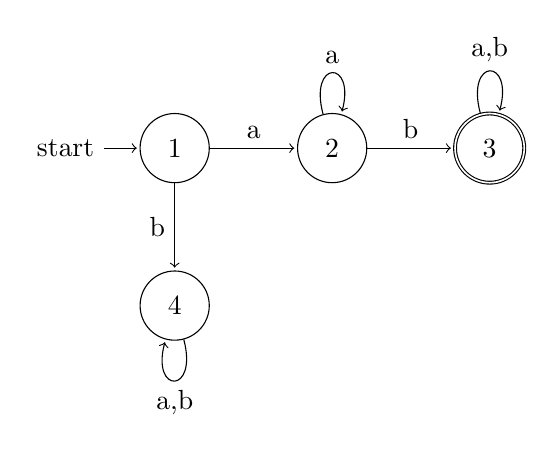
\begin{tikzpicture}[shorten >=1pt, node distance=2cm, on grid, auto] 

   \node[state, initial] (q1) {1}; 
   \node[state] (q2) [right=of q1] {2}; 
   \node[state, accepting] (q3) [right=of q2] {3}; 
   \node[state] (q4) [below=of q1] {4}; 

    \path[->]
    (q1) edge [above] node {a} (q2)
         edge [left]  node {b} (q4)
    (q2) edge [loop above] node {a} ()
         edge [above] node {b} (q3)
    (q3) edge [loop above] node {a,b} ()
    (q4) edge [loop below] node {a,b} ();
\end{tikzpicture}
\end{center}


\begin{center}
\textbf{DFA $A_2$}
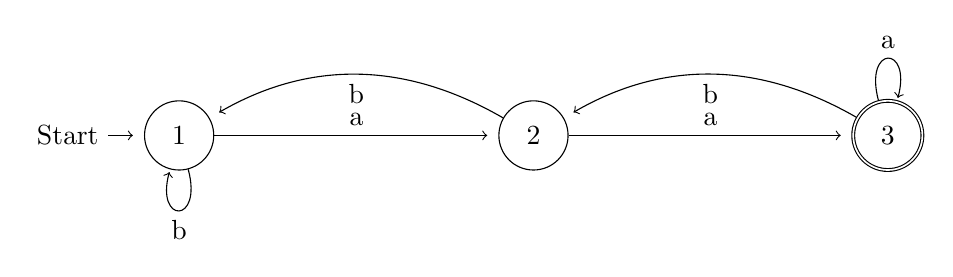
\begin{tikzpicture}[shorten >=4pt, node distance=4.5cm, on grid, auto] 

   \node[state, initial, initial text=Start] (q1) {1}; 
   \node[state] (q2) [right=of q1] {2}; 
   \node[state, accepting] (q3) [right=of q2] {3}; 

    \path[->]
    (q1) edge [above] node {a} (q2)
         edge [loop below] node {b} ()
    (q2) edge [above] node {a} (q3)
         edge [bend right=30, below] node {b} (q1)
    (q3) edge [loop above] node {a} ()
         edge [bend right=30, below] node {b} (q2);
\end{tikzpicture}
\end{center}


\textbf{Words accepted or refused by $\mathcal A_1$ and $\mathcal A_2$, respectively}
\[
\begin{array}{c|c|c}
w & \text{Accepted } A_1 & \text{Accepted } A_2 \\ \midrule
aaa & \textcolor{red}{\times} & \textcolor{green}{\checkmark} \\
aab & \textcolor{green}{\checkmark} & \textcolor{red}{\times} \\
aba & \textcolor{red}{\times} & \textcolor{red}{\times} \\
abb & \textcolor{red}{\times} & \textcolor{red}{\times} \\
baa & \textcolor{red}{\times} & \textcolor{green}{\checkmark} \\
bab & \textcolor{red}{\times} & \textcolor{red}{\times} \\
bba & \textcolor{red}{\times} & \textcolor{red}{\times} \\
bbb & \textcolor{red}{\times} & \textcolor{red}{\times} \\
\end{array}
\]
\noindent The table above summarizes the words accepted or rejected by DFA $A_1$ and DFA $A_2$. 
To implement these automata \textit{programmatically}, we define the DFA class in \texttt{dfa.py}, which allows us to process input words according to their respective state transition diagrams.

\textbf{\text{DFA Implementation in \texttt{dfa.py}}}\\
This introduction describes the design of the \texttt{dfa.py},  consisting of:
\begin{itemize}
  \item$Q$ - a finite set of states.
  \item$\Sigma$ - an input alphabet.
  \item$\delta : Q \times \Sigma \to Q$ - a transition function.
  \item$q_0 \in Q$ an initial state.
  \item$F \subseteq Q$ - a set of final accepting states.
\end{itemize}

The \texttt{DFA} class constructor takes these five elements (\texttt{Q}, \texttt{Sigma}, \texttt{delta}, \texttt{q0}, and \texttt{F}), using the method:
\begin{itemize}
  \item \texttt{run(w)}: Runs the DFA on input string \texttt{w} and determines whether or not \texttt{w} is accepted based on the state it finishes at.
\end{itemize}

\textbf{Implementation}
In the following code snippet, the \texttt{run} method processes the symbols of the input \texttt{w} sequentially, looking up the next state based on the current state and the input symbol. If an invalid transition is encountered, the method immediately returns \texttt{False}. Otherwise, if the DFA ends in a state that is a member of \texttt{F}, \texttt{True} is returned (meaning \texttt{w} is accepted); if it ends in some other state, \texttt{False} is returned.

\begin{lstlisting}
class DFA :

    # init the DFA
    def __init__(self, Q, Sigma, delta, q0, F) : 
        self.Q = Q # set of states
        self.Sigma = Sigma # set of symbols
        self.delta = delta # transition function
        self.q0 = q0 # initial state
        self.F = F # final states
   
   # print the data of the DFA
    def __repr__(self) :
        return f"DFA({self.Q},\n\t{self.Sigma},\n\t{self.delta},\n\t{self.q0},\n\t{self.F})"

    # run the DFA on the word w
    # return if the word is accepted or not
    # modify as needed
    def run(self, w) :
        # todo
        # start at initial state
        current_state = self.q0
        for symbol in w:
            if (current_state, symbol) in self.delta:
                current_state = self.delta[(current_state, symbol)]
            else:
                # invalid transition (dead state)
                return False
            # accept if in final state
        return current_state in self.F 

\end{lstlisting}

\textbf{Exercise 4: A new automaton from an old one}

Below is DFA $A_0$ which accepts exactly the words that $A$ refuses and vice versa.
\begin{center}
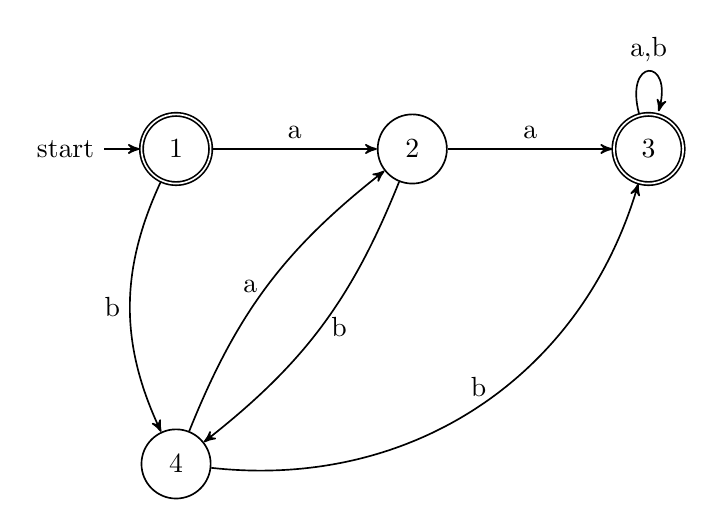
\begin{tikzpicture}[->, >=stealth', auto, semithick]
  \node[state, initial, accepting]      (q1) at (0,0)   {1};
  \node[state]                          (q2) at (3,0)   {2};
  \node[state, accepting]               (q3) at (6,0)   {3};
  \node[state]                          (q4) at (0,-4){4};
  \path
    % 1 -> 2, labeled 'a'
    (q1) edge                node[above] {a} (q2)
    % 1 -> 4, labeled 'b'
    (q1) edge[bend right=25] node[left]  {b} (q4)
    % 2 -> 3, labeled 'a'
    (q2) edge                node[above] {a} (q3)
    % 2 -> 4, labeled 'b'
    (q2) edge[bend left=15] node[right] {b} (q4)
    % 4 -> 2, labeled 'a'
    (q4) edge[bend left=15]  node[left]  {a} (q2)
    % 4 -> 3, labeled 'b'
    (q4) edge[bend right=40]  node[above] {b} (q3)
    % 3 -> 3 loop, labeled 'a,b'
    (q3) edge[loop above]    node        {a,b} ();

\end{tikzpicture}
\end{center}
In $A_0$, nodes 1 and 3 are the accepting final states, while nodes 2 and 4 are normal states.

\textbf{Exercise 2.2.4: DFAs over $\{0,1\}$}

{(a) The set of all strings ending in 00}

\noindent
\textbf{DFA Description:}
\[
\begin{aligned}
Q &= \{\,q_0,\, q_1,\, q_2\},\\
\Sigma &= \{0,1\},\\
\delta &\text{ is given by the table below},\\
q_0 &\text{ is the start state},\\
F &= \{\,q_2\}.
\end{aligned}
\]

\noindent
\textbf{Transition Table:}
\[
\begin{array}{c|cc}
  \delta & 0 & 1 \\
\hline
  q_0    & q_1 & q_0 \\
  q_1    & q_2 & q_0 \\
  q_2    & q_2 & q_0
\end{array}
\]

\noindent
\textit{Explanation:} 
\begin{itemize}
\item $q_0$ - we have not yet seen a trailing zero
\item $q_1$ - the string currently ends in exactly one zero
\item $q_2$ (accepting) - the string ends in at least two consecutive zeros
\end{itemize}

\bigskip

{(b) The set of all strings with three consecutive 0s}

\noindent
\textbf{DFA Description:}
\[
\begin{aligned}
Q &= \{\,q_0,\, q_1,\, q_2,\, q_3\},\\
\Sigma &= \{0,1\},\\
\delta &\text{ is given by the table below},\\
q_0 &\text{ is the start state},\\
F &= \{\,q_3\}.
\end{aligned}
\]

\noindent
\textbf{Transition Table:}
\[
\begin{array}{c|cc}
  \delta & 0 & 1 \\
\hline
  q_0    & q_1 & q_0 \\
  q_1    & q_2 & q_0 \\
  q_2    & q_3 & q_0 \\
  q_3    & q_3 & q_3
\end{array}
\]

\noindent
\textit{Explanation:}
\begin{itemize}
\item $q_0$ - we have seen 0 consecutive zeros so far
\item $q_1$ - we have seen exactly 1 consecutive zero
\item $q_2$ - we have seen exactly 2 consecutive zeros
\item $q_3$ (accepting) - we have seen at least 3 consecutive zeros
\end{itemize}

\bigskip

{(c) The set of all strings with \texttt{011} as a substring}

\noindent
\textbf{DFA Description:}
\[
\begin{aligned}
Q &= \{\,q_0,\, q_1,\, q_2,\, q_3\},\\
\Sigma &= \{0,1\},\\
\delta &\text{ is given by the table below},\\
q_0 &\text{ is the start state},\\
F &= \{\,q_3\}.
\end{aligned}
\]

\noindent
\textbf{Transition Table:}
\[
\begin{array}{c|cc}
  \delta & 0 & 1 \\
\hline
  q_0    & q_1 & q_0 \\
  q_1    & q_1 & q_2 \\
  q_2    & q_1 & q_3 \\
  q_3    & q_3 & q_3
\end{array}
\]

\noindent
\textit{Explanation:}
\begin{itemize}
\item $q_0$ - no partial match yet
\item $q_1$ - we matched a single \texttt{0}
\item $q_2$ - we matched \texttt{01}
\item $q_3$ (accepting) - we found \texttt{011} somewhere in the string
\end{itemize}
\bigskip

\subsection{\textbf{Week 4}}\\
\textbf{Lecture Summary}\\
%Summarize when I get the chance
We explore the concept of \emph{product automata} and how they can be used to model operations on languages accepted by two deterministic finite automata (DFAs). In particular, we discuss how to construct an automaton that accepts the intersection (or union) of the languages recognized by two given automata.

\textbf{Homework 3}

\textbf{Problem 1: Extended transition function}\\
Consider two DFAs:
\[
\mathcal{A}^{(1)} = \big(Q^{(1)}, \Sigma, \delta^{(1)}, q_0^{(1)}, F^{(1)}\big) \quad \text{and} \quad \mathcal{A}^{(2)} = \big(Q^{(2)}, \Sigma, \delta^{(2)}, q_0^{(2)}, F^{(2)}\big),
\] 
\\over the alphabet $\Sigma = \{a, b\}$.
\begin{center}
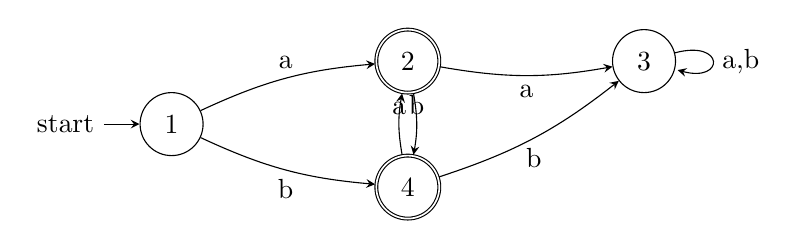
\begin{tikzpicture}[>=stealth,node distance=2.5cm,on grid,auto]
\tikzstyle{state}=[circle,draw,minimum size=8mm,inner sep=0pt]

  %--- nodes ---
  \node[state, initial] (1) {1};
  \node[state, accepting] (2) [right=3cm of 1, yshift=0.8cm] {2};
  \node[state, accepting] (4) [right=3cm of 1, yshift=-0.8cm] {4};
  \node[state] (3) [right=3cm of 2] {3};

  %--- transitions ---
  \path[->]
    (1) edge[bend left=10] node[above] {a} (2)
    (1) edge[bend right=10] node[below] {b} (4)

    (2) edge[bend left=10] node[above] {b} (4)
    (2) edge[bend right=10] node[below] {a} (3)

    (4) edge[bend left=10] node[above] {a} (2)
    (4) edge[bend right=10] node[below] {b} (3)

    (3) edge[loop right] node {a,b} (3);
\end{tikzpicture}
\end{center}

\noindent
\textit{Diagram for \(A^{(1)}\):}
\begin{itemize}
  \item State 1 is the initial state (arrow from the left).
  \item From state 1: reading `\(a\)' goes to 2; reading `\(b\)' goes to 4.
  \item From state 2: reading `\(a\)' goes to 3; reading `\(b\)' goes to 4.
  \item From state 4: reading `\(a\)' goes to 2; reading `\(b\)' goes to 3.
  \item From state 3: reading either `\(a\)' or `\(b\)' loops on 3.
  \item States 2 and 4 are accepting, while state 3 is a non-accepting sink.
\end{itemize}

\bigskip

\begin{center}
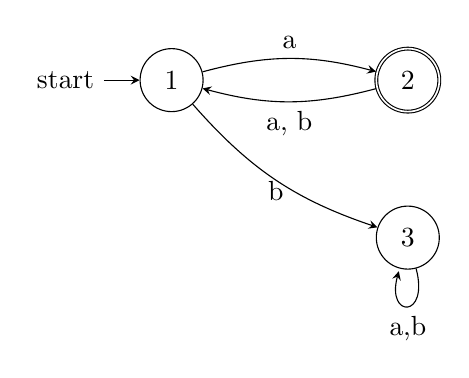
\begin{tikzpicture}[>=stealth,node distance=2.5cm,on grid,auto]
\tikzstyle{state}=[circle,draw,minimum size=8mm,inner sep=0pt]

%--- nodes ---
\node[state, initial] (1) {1};
\node[state, accepting] (2) [right=3cm of 1] {2};
\node[state] (3) [below=2cm of 2] {3};

%--- initial arrow ---
\path[->] 
  node[above left=0.5cm of 1]{}
  (1);

%--- transitions ---
\path[->]
  (1) edge[bend left=15] node[above] {a} (2)
  (1) edge[bend right=15] node[left,pos=0.6] {b} (3)
  (2) edge[bend left=15] node[below] {a, b} (1)
  (3) edge[loop below] node {a,b} (3);

\end{tikzpicture}
\end{center}

\noindent
\textit{Diagram for \(A^{(2)}\):}
\begin{itemize}
  \item State 1 is the initial state (arrow from the left).
  \item From state 1: reading `\(a\)' goes to 2; reading `\(b\)' goes to 3.
  \item From state 2: reading `\(a\)' or `\(b\)' goes back to 1.
  \item State 3 loops on both `\(a\)' and `\(b\)'.
  \item State 2 is the only accepting state.
\end{itemize}

\textbf{a. Descriptions of Accepted Languages}

\begin{itemize}
    \item \textbf{$\mathcal{A}^{(1)}$:} Accepts non-empty words in which no two consecutive letters are the same.
    \item \textbf{$\mathcal{A}^{(2)}$:} Accepts words of odd length where every letter at an odd position of $w$ is the letter $a$.
\end{itemize}
Hence,
\[
L\bigl(A^{(2)}\bigr)
=\bigl\{\,w \in \{a,b\}^* \,\mid\, |w|\text{ is odd and the odd-indexed letters are all }a\bigr\}.
\]

\bigskip

\textbf{b. Computation: $\widehat{\delta}^{(1)}\bigl(1,\texttt{abaa}\bigr)$}

The automaton $A^{(1)}$ has states $\{1,2,3,4\}$, where:
\begin{itemize}
    \item State 1 is the initial state (non-final).
    \item State 2 indicates the last letter read was $a$ (no violation).
    \item State 4 indicates the last letter read was $b$ (no violation).
    \item State 3 is the ``sink'' or ``trap'' state (once a violation occurs, e.g.\ two consecutive letters the same).
\end{itemize}
We compute step-by-step for the input \(\texttt{abaa}\):
\[
\widehat{\delta}^{(1)}(1,\texttt{abaa}):
\]
\begin{enumerate}
    \item Start in state $1$, input = \texttt{abaa}.
    \item Read `a': $\delta^{(1)}(1,a) = 2$. Remaining input = \texttt{baa}.
    \item Now in state $2$, read `b': $\delta^{(1)}(2,b) = 4$. Remaining input = \texttt{aa}.
    \item Now in state $4$, read `a': $\delta^{(1)}(4,a) = 2$. Remaining input = \texttt{a}.
    \item Now in state $2$, read `a': $\delta^{(1)}(2,a) = 3$. Remaining input is empty.
\end{enumerate}
Therefore,
\[
\widehat{\delta}^{(1)}(1,\texttt{abaa}) \;=\; 3.
\]
Since state $3$ is the non-accepting sink, the string \texttt{abaa} is not accepted by $A^{(1)}$.

\bigskip

\textbf{b. Computation: $\widehat{\delta}^{(2)}\bigl(1,\texttt{abba}\bigr)$}

Automaton $A^{(2)}$ can be thought of as having states:
\begin{itemize}
    \item State 1: an even number of letters read so far (initial, non-final).
    \item State 2: an odd number of letters read so far, with ``odd positions must be $a$'' still satisfied (accepting).
    \item State 3: dead/trap state (if the condition on odd positions is violated).
\end{itemize}
We compute for \(\texttt{abba}\) (positions are 1,2,3,4):
\[
\widehat{\delta}^{(2)}(1,\texttt{abba}):
\]
\begin{enumerate}
    \item Start in state $1$, input = \texttt{abba}.
    \item Read `a' (position 1): $\delta^{(2)}(1,a) = 2$. Remaining input = \texttt{bba}.
    \item Now in state $2$, read `b' (position 2): $\delta^{(2)}(2,b) = 1$. Remaining input = \texttt{ba}.
    \item Now in state $1$, read `b' (position 3): $\delta^{(2)}(1,b) = 3$. Remaining input = \texttt{a}.
    \item Now in state $3$, read `a': $\delta^{(2)}(3,a) = 3$. Remaining input is empty.
\end{enumerate}
Hence,
\[
\widehat{\delta}^{(2)}(1,\texttt{abba}) = 3,
\]
and state $3$ is non-accepting. Therefore, \texttt{abba} is not accepted by $A^{(2)}$.

\bigskip

\textbf{Problem 2: Product automata}

We now define a \emph{product automaton} $A$ from $A^{(1)}$ and $A^{(2)}$ in order to recognize 
\[
L\bigl(A^{(1)}\bigr) \;\cap\; L\bigl(A^{(2)}\bigr).
\]

\subsubsection*{a. Construct the intersection automaton $A$}

\noindent \textbf{States.} The state set of $A$ is the Cartesian product
\[
Q \;=\; Q^{(1)} \;\times\; Q^{(2)}.
\]
If $Q^{(1)} = \{1,2,3,4\}$ and $Q^{(2)} = \{1,2,3\}$, then
\[
Q = \{(1,1),(1,2),(1,3),(2,1),(2,2),(2,3),(3,1),(3,2),(3,3),(4,1),(4,2),(4,3)\}.
\]

\noindent \textbf{Initial state.} $(1,1)$, since $1$ is the initial state of $A^{(1)}$ and $1$ is the initial state of $A^{(2)}$.

\noindent \textbf{Transition function.} For $(p,q)\in Q$ and $x \in \{a,b\}$,
\[
\delta\bigl((p,q),x\bigr) \;=\; \bigl(\delta^{(1)}(p,x),\;\delta^{(2)}(q,x)\bigr).
\]

\noindent \textbf{Final states (for intersection).} A pair $(p,q)$ is final if $p \in F^{(1)}$ and $q \in F^{(2)}$. 
- For $A^{(1)}$, we have $F^{(1)} = \{2,4\}$ (all non-empty strings with no two consecutive letters the same).  
- For $A^{(2)}$, we have $F^{(2)} = \{2\}$ (odd-length strings with \(a\) in every odd position).

Thus
\[
F \;=\; \{(p,q) \mid p \in \{2,4\},\, q = 2\}.
\]

\paragraph{Diagram of product automaton $A$}showing all transitions. For brevity, not every state is drawn if some are unreachable.

\begin{center}
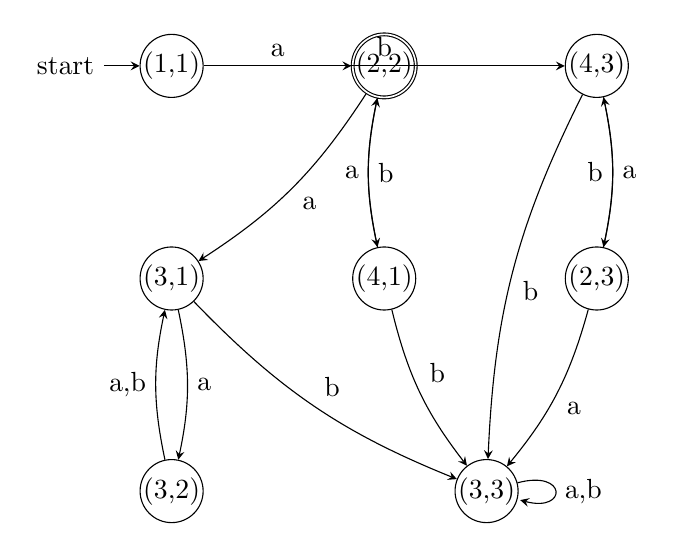
\begin{tikzpicture}[>=stealth,node distance=2.7cm,on grid,auto]
\tikzstyle{state}=[circle,draw,minimum size=8mm,inner sep=0pt]

%-- Nodes that are reachable only  --
\node[state, initial] (11) {(1,1)};
\node[state, accepting] (22) [right of=11] {(2,2)};
\node[state] (43) [right of=22] {(4,3)};
\node[state] (31) [below of=11] {(3,1)};
\node[state] (41) [below of=22] {(4,1)};
\node[state] (23) [below of=43] {(2,3)};
\node[state] (32) [below of=31] {(3,2)};
\node[state] (33) [below of=41, xshift=1.3cm] {(3,3)};

%-- Transitions --
\path[->]
  % (1,1)
  (11) edge node {a} (22)
  (11) edge node {b} (43)

  % (2,2)
  (22) edge[bend left=12] node {a} (31)
  (22) edge[bend right=12] node {b} (41)

  % (4,3)
  (43) edge[bend left=12] node {a} (23)
  (43) edge[bend right=12] node {b} (33)

  % (3,1)
  (31) edge[bend left=12] node {a} (32)
  (31) edge[bend right=12] node {b} (33)

  % (4,1)
  (41) edge[bend left=12] node {a} (22)
  (41) edge[bend right=12] node {b} (33)

  % (2,3)
  (23) edge[bend left=12] node {a} (33)
  (23) edge[bend right=12] node {b} (43)

  % (3,2)
  (32) edge[bend left=12] node {a,b} (31)

  % (3,3)
  (33) edge[loop right] node {a,b} (33);

\end{tikzpicture}
\end{center}

\subsubsection*{b. Why $L(A) = L\bigl(A^{(1)}\bigr)\,\cap\,L\bigl(A^{(2)}\bigr)$}

A string $w$ is accepted by $A$ precisely if:
\begin{itemize}
    \item Following the transitions of $A$ on $w$ leads from $(1,1)$ to a final state $(p,q)$.
    \item This happens exactly when $p$ is a final state of $A^{(1)}$ \emph{and} $q$ is a final state of $A^{(2)}$.
\end{itemize}
Thus $w$ is accepted by both $A^{(1)}$ and $A^{(2)}$. Hence $L(A) = L(A^{(1)}) \cap L(A^{(2)})$.

\subsubsection*{c. Constructing $A'$ for the Union}

To get $L(A') = L\bigl(A^{(1)}\bigr) \cup L\bigl(A^{(2)}\bigr)$, we keep the same product structure but change the final states. A product state $(p,q)$ is final if \emph{either} $p \in F^{(1)}$ \emph{or} $q \in F^{(2)}$. Formally:
\[
F' \;=\; \bigl(F^{(1)} \times Q^{(2)}\bigr) \;\cup\;\bigl(Q^{(1)} \times F^{(2)}\bigr).
\]
This ensures that a string is accepted by $A'$ if it is accepted by $A^{(1)}$ \emph{or} $A^{(2)}$.

\bigskip

\noindent \textbf{Summary of Key Points:}
\begin{itemize}
    \item For $A^{(1)}$, the accepting states are $\{2,4\}$; consecutive letters must differ and the string must be non-empty.
    \item For $A^{(2)}$, the accepting state is $\{2\}$; the string must have odd length and $a$ in every odd position.
    \item Extended transitions showed that $\widehat{\delta}^{(1)}(1,\texttt{abaa}) = 3$ (not accepted) and $\widehat{\delta}^{(2)}(1,\texttt{abba}) = 3$ (not accepted).
    \item The product automaton for intersection has final states $F^{(1)} \times F^{(2)} = \{(2,2), (4,2)\}$, while for union we use $F' = (F^{(1)} \times Q^{(2)}) \;\cup\; (Q^{(1)} \times F^{(2)})$.
\end{itemize}
\bigskip\bigskip\bigskip\bigskip\bigskip\bigskip\bigskip\bigskip\bigskip\bigskip\bigskip\bigskip

\textbf{Exercise 2.2.7: Induction Proof}

\noindent
\textbf{Statement:} Let $A$ be a DFA, and let $q$ be a particular state of $A$ such that
\[
\delta(q,a) \;=\; q
\quad
\text{for all input symbols } a.
\]
Show by induction on the length of the input that for all input strings $w$, we have
\[
\widehat{\delta}(q,w) \;=\; q.
\]

\bigskip

\noindent
\textbf{Proof (by induction on the length of $w$):}

\paragraph{Base Case ($|w| = 0$):}
If $w$ is the empty string $\epsilon$, then by definition of the extended transition function,
\[
\widehat{\delta}(q,\epsilon) \;=\; q.
\]
Hence the statement holds for $|w| = 0$.

\paragraph{Inductive Step:}
Assume that for all strings $x$ of length $n$, we have
\[
\widehat{\delta}(q,x) \;=\; q.
\]
We need to prove the statement for any string $w$ of length $n+1$. Let $w$ be such a string. We can write $w$ as
\[
w \;=\; x\,a,
\]
where $x$ is a string of length $n$, and $a$ is a single input symbol. Then,
\[
\widehat{\delta}(q,w)
\;=\;
\widehat{\delta}(q,\,x\,a)
\;=\;
\delta\bigl(\widehat{\delta}(q,x),\,a\bigr).
\]
By the inductive hypothesis, $\widehat{\delta}(q,x) = q$. Therefore,
\[
\widehat{\delta}(q,w)
\;=\;
\delta(q,a).
\]
But we are given that $\delta(q,a) = q$ for all symbols $a$. Hence,
\[
\widehat{\delta}(q,w)
\;=\;
q.
\]
This completes the inductive step.

\paragraph{Conclusion:}
By the principle of mathematical induction, for all strings $w$, we have
\[
\widehat{\delta}(q,w) = q.
\]
Thus, if a state $q$ transitions to itself on every symbol, it remains $q$ under any input string.
\paragraph{ITALC 2.3 Question:}
In the subset construction for converting an NFA to a DFA, often there is an exponential blow-up in the number of states. Can you propose a scenario for which this blow-up actually happens, and whether there are any strategies or special cases that might mitigate this worst-case behavior?

\subsection{\textbf{Week 5}}\\
\textbf{Lecture Summary}\\
%Summarize when I get the chance
TBD

\textbf{Homework 4}\\
\textbf{Problem 1: NFA Interpretation}
We can consider $A$ as an NFA because each transition goes to a 
single-element set (instead of exactly one state). Hence, $A$ 
can be viewed as a valid NFA.

\[
A' = \bigl(Q', \Sigma, \delta', q'_0, F'\bigr),
\]
where
\[
Q' = Q, 
\quad
q'_0 = q_0, 
\quad
F' = F,
\quad
\delta'(q,a) = \{\delta(q,a)\}.
\]

\textbf{2. Why it works.}

Each string accepted by $A$ has the exact same single path of states 
in $A'$, because $\delta'$ uses the same transitions as $\delta$, 
but returns them as singleton sets. 
Thus, every string accepted by $A'$ follows that same single path of 
states in $A$. Consequently,
\[
L(A') \;=\; L(A).
\]

\textbf{Problem 2: }
The NFA $A$ has four states $q_0, q_1, q_2, q_3$, with $q_0$ as the 
start state and $q_3$ as the (only) accepting state. The transitions are:
\[
\delta(q_0,0) = \{q_1\}, \quad
\delta(q_0,1) = \{q_1\},
\]
\[
\delta(q_1,0) = \{q_2\}, \quad
\delta(q_1,1) = \{q_2, q_3\},
\]
\[
\delta(q_2,0) = \varnothing, \quad
\delta(q_2,1) = \{q_3\},
\]
\[
\delta(q_3,0) = \varnothing, \quad
\delta(q_3,1) = \varnothing.
\]

There are no loops, so only strings of length $2$ or $3$ can reach $q_3$. 
Specifically:
\begin{itemize}
\item For length $2$: 
  \[
    q_0 \xrightarrow{\,0\text{ or }1\,} q_1 
    \xrightarrow{\,1\,} q_3,
  \]
  which corresponds to the strings $\{01,\,11\}$.
\item For length $3$:
  \[
    q_0 \xrightarrow{\,0\text{ or }1\,} q_1
    \xrightarrow{\,0\text{ or }1\,} q_2
    \xrightarrow{\,1\,} q_3,
  \]
  which corresponds to the strings $\{001,\,011,\,101,\,111\}$.
\end{itemize}

Hence, the language is:
\[
L(A) \;=\; \{\,01,\,11,\,001,\,011,\,101,\,111\}.
\]

\subsection*{2. Specify $A$ in the form $(Q,\Sigma,\delta,q_0,F)$}

\[
Q = \{q_0,\, q_1,\, q_2,\, q_3\}, \quad
\Sigma = \{0,1\}, \quad
q_0 \text{ is the start state}, \quad
F = \{q_3\}.
\]
The transition function $\delta$ is as above.

\subsection*{3. Compute $\hat{\delta}\bigl(q_0,\,10110\bigr)$ step by step}

We track the set of possible states after each input symbol:

\begin{enumerate}
\item Start: $\{q_0\}$.
\item Read `1`: $\delta(q_0,1) = \{q_1\}$, so now in $\{q_1\}$.
\item Read `0`: $\delta(q_1,0) = \{q_2\}$, so now in $\{q_2\}$.
\item Read `1`: $\delta(q_2,1) = \{q_3\}$, so now in $\{q_3\}$.
\item Read `1`: $\delta(q_3,1) = \varnothing$, so now in $\varnothing$.
\item Read `0`: from $\varnothing$, we stay in $\varnothing$.
\end{enumerate}

Thus,
\[
\hat{\delta}(q_0,\,10110) \;=\; \varnothing.
\]
Since $\varnothing$ does not contain a final state, $10110$ is not accepted.

\subsection*{4. Find all paths in $A$ for $v = 1$ and $w = 1010$}

\paragraph{For $v = 1$:}
\[
q_0 \xrightarrow{\,1\,} q_1.
\]
No more input; we end in $q_1$. Since $q_1 \notin F$, the string $1$ is 
not accepted.

\paragraph{For $w = 1010$:}
\[
q_0 \xrightarrow{\,1\,} q_1 
\xrightarrow{\,0\,} q_2 
\xrightarrow{\,1\,} q_3 
\xrightarrow{\,0\,} \varnothing.
\]
We end in $\varnothing$, so $1010$ is not accepted. 
In both cases, there is a unique path because the transitions 
are forced by the input symbols.

\subsection*{5. Construct the determinization $A^D$ (power-set construction)}

We list the reachable subsets of $\{q_0, q_1, q_2, q_3\}$:

\begin{itemize}
\item \textbf{Start state}: $\{q_0\}$. 
  \begin{itemize}
  \item On $0$ or $1$, go to $\{q_1\}$.
  \end{itemize}
\item \textbf{State} $\{q_1\}$.
  \begin{itemize}
  \item On $0$: $\{q_2\}$.
  \item On $1$: $\{q_2,q_3\}$.
  \end{itemize}
\item \textbf{State} $\{q_2\}$.
  \begin{itemize}
  \item On $0$: $\varnothing$.
  \item On $1$: $\{q_3\}$.
  \end{itemize}
\item \textbf{State} $\{q_2,q_3\}$.
  \begin{itemize}
  \item On $0$: $\varnothing$.
  \item On $1$: $\{q_3\}$.
  \end{itemize}
\item \textbf{State} $\{q_3\}$.
  \begin{itemize}
  \item On $0$: $\varnothing$.
  \item On $1$: $\varnothing$.
  \end{itemize}
\item \textbf{Dead state} $\varnothing$.
  \begin{itemize}
  \item On $0$ or $1$: $\varnothing$.
  \end{itemize}
\end{itemize}

The start state in the DFA is $\{q_0\}$, and the accepting states are 
all subsets containing $q_3$, namely $\{q_2,q_3\}$ and $\{q_3\}$.

\subsection*{6. Verify $L(A) = L(A^D)$. Is there a smaller DFA?}

By the standard subset construction, we have $L(A^D) = L(A)$. 
Since $L(A)$ is the finite set of strings $\{01,\,11,\,001,\,011,\,101,\,111\}$, 
one might suspect a smaller DFA could exist. However, standard DFA 
minimization shows that all the reachable states in $A^D$ are pairwise 
inequivalent, so no merges are possible without altering the language. 
Hence, the $6$-state DFA is already minimal.

\textbf{Question:} Can you describe a practical scenario where combining the two (i.e  first designing an NFA and then converting or integrating it into a DFA) provides benefits that neither approach alone can normally offer?



\end{document}


\section{Synthesis}

\section{Evidence of Participation}

\section{Conclusion}\label{conclusion}

\begin{thebibliography}{99}
\bibitem[BLA]{bla} Author, \href{https://en.wikipedia.org/wiki/LaTeX}{Title}, Publisher, Year.
\end{thebibliography}

\end{document}